\documentclass[xcolor=table]{beamer}

\mode<presentation> {
\usetheme{Madrid}
}

\usepackage{graphicx}
\usepackage[utf8]{inputenc} 
\usepackage[french]{babel}

\usepackage{multirow}
\usepackage[table]{xcolor}

\title{Authentification \`{a} base d'OTP}
\author{M1SSI}
\institute[Université de Rouen] {
Université de Rouen \\
\medskip
}
\date{\today}

\AtBeginSubsection[] 
{ 
\begin{frame}  
\frametitle{Plan} 
\tableofcontents[currentsubsection,hideothersubsections,subsectionstyle=show/shaded]
\end{frame}
} 

%------------------------------------------
\begin{document}
\begin{frame}
\titlepage
\end{frame}

\begin{frame}
\frametitle{Table des matières}
\tableofcontents
\end{frame}

%------------------------------------------------
\section{Introduction}
%------------------------------------------------
\subsection{Au commencement}
\begin{frame}
\frametitle{L'équipe}
\begin{block}{Le chef}
Adrien \bsc{Smondack}.
\end{block}
\begin{block}{La technique}
Yves \bsc{Adegoloye} et Damien \bsc{Picard}.
\end{block}
\begin{block}{La qualité}
Claire \bsc{Hardouin} et Gaëtan \bsc{Ferry}.
\end{block}
\begin{block}{La MOA}
Maxime \bsc{Michotte} et Benjamin \bsc{Zigh}.
\end{block}
\end{frame}


\begin{frame}
\frametitle{Le projet}

\begin{block}{Clients}
\begin{description}
\item[Magali \bsc{Bardet}:] Enseignante-Chercheuse à l'université de Rouen.\\
\item[Bruno \bsc{Macadré}:] Ingénieur Système à l'université de Rouen.
\end{description}
\end{block}

\begin{block}{Sujet}
Création d'un système d'authentification à base de mots de passe jetables.
\end{block}
\end{frame}

\subsection{Authentification classique}
\begin{frame}
\frametitle{Exemple}
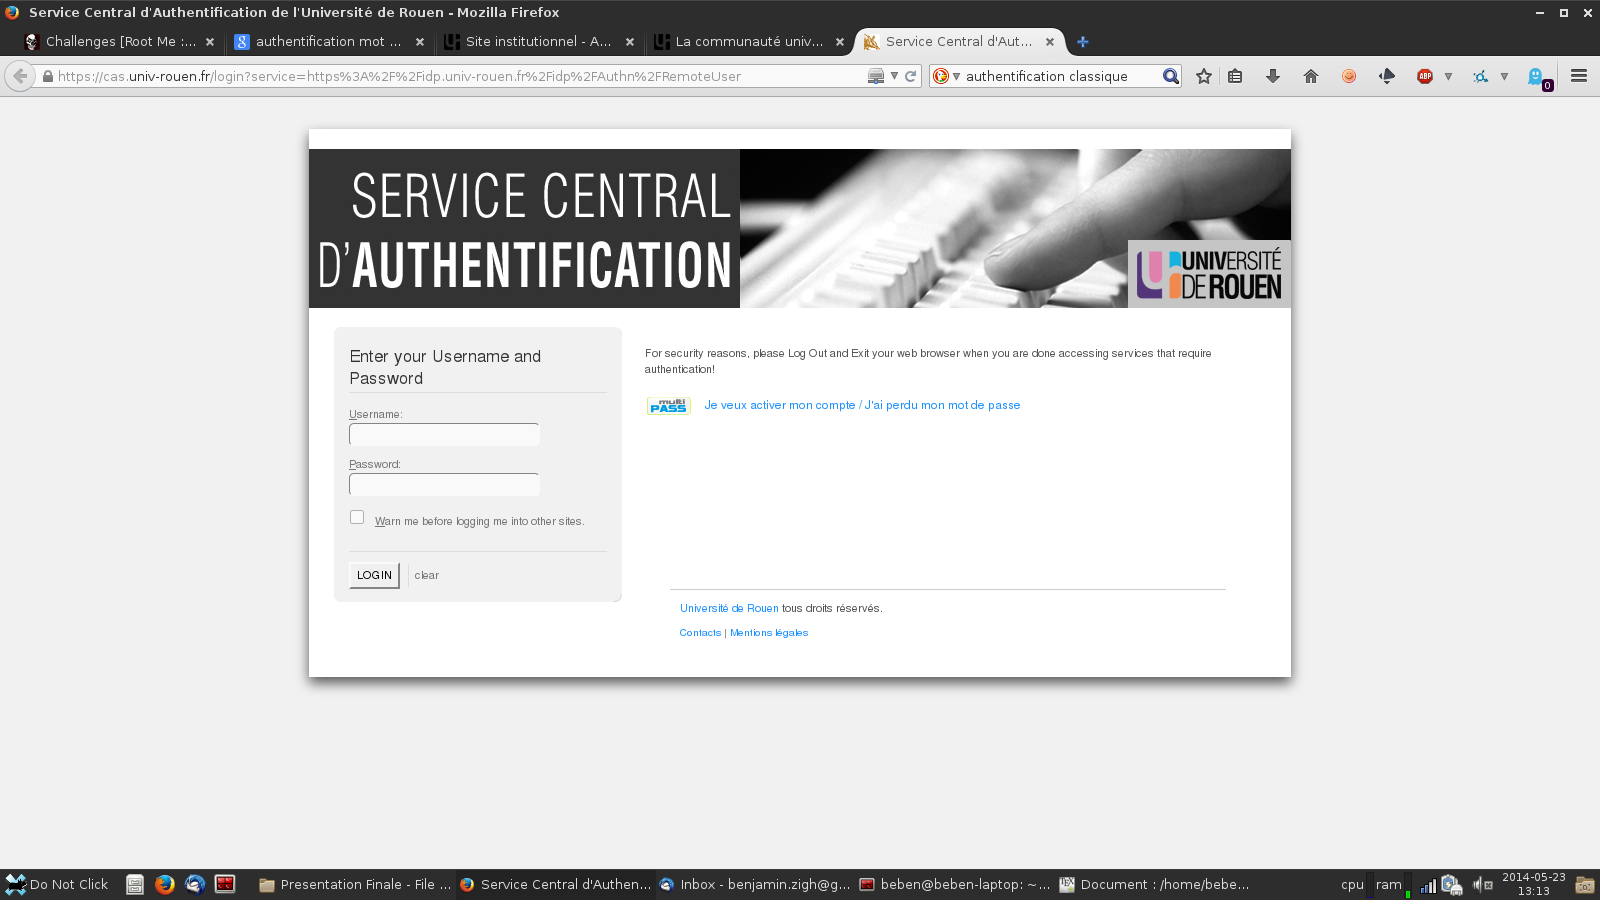
\includegraphics[scale=0.21]{../graphics/auth-mdp.png}
\end{frame}

\begin{frame}
\frametitle{Principe de base}
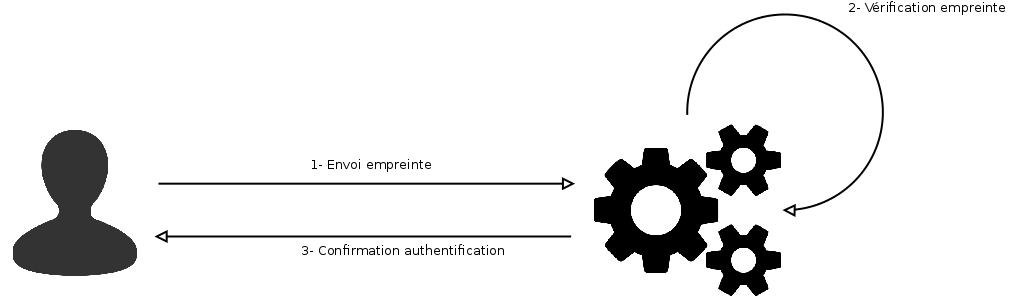
\includegraphics[scale=0.24]{../graphics/authsimple.png}
\end{frame}

\subsection{Authentification OTP}
\begin{frame}
\frametitle{Exemples}
\begin{center}
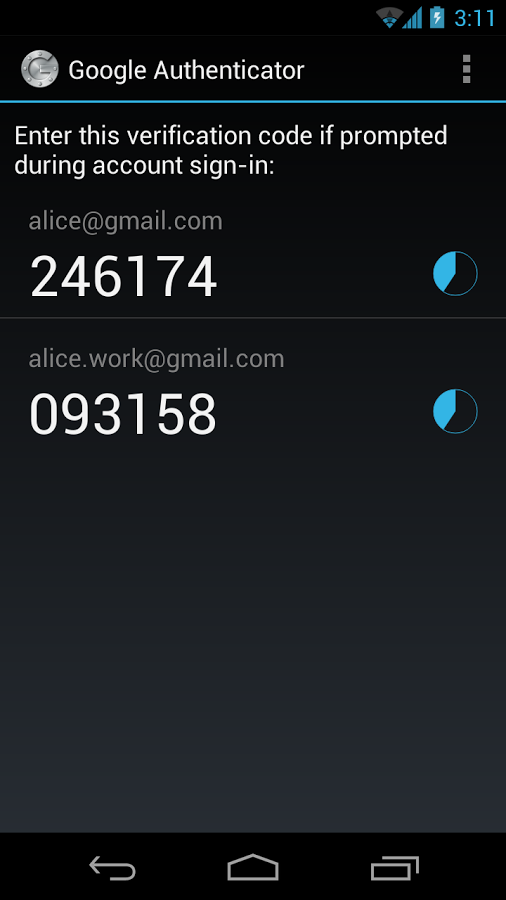
\includegraphics[scale=0.2]{../graphics/googleauth.png}
\hspace{1em}
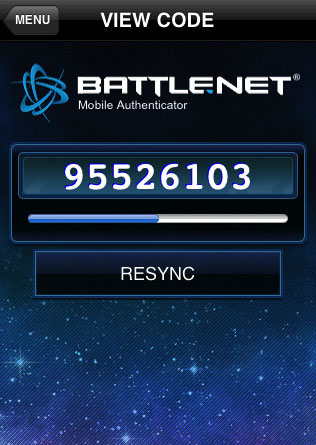
\includegraphics[scale=0.405]{../graphics/blizzardauth.jpg}
\end{center}
\end{frame}

\begin{frame}
\frametitle{Principe OTP}
%Schéma OTP à modifier
haha
\end{frame}


\begin{frame}
\frametitle{Avantages de l'OTP}
\begin{block}{Définition}
    Un OTP est un mot de passe jetable, c'est à dire qu'il satisfait les deux 
  critères suivants:
  \begin{itemize}
    \item Il n'est pas prévisible
    \item Il n'est valide que pour une unique session.
  \end{itemize}
\end{block}

\begin{block}{Utilité}
  \begin{itemize}
    \item Permettre une authentification à 2 facteurs (\og{} forte\fg{}).
    \item Éviter les attaques par rejeu.
  \end{itemize}
\end{block}
\end{frame}

%--------------------------------------
\section{Le Projet}

\subsection{Demande du client}

\begin{frame}
\frametitle{Les livrables}
\begin{block}{État de l'art} 
Un état de l'art comprenant au moins trois protocoles OTP étudiés.
\end{block}
\begin{block}{Équipes de recherche}
  \begin{itemize}
    \item EAP-POTP
    \begin{itemize}
      \item Tayewo-John-Yves \bsc{Adegoloye}
      \item Claire \bsc{Hardouin}
    \end{itemize}
    \item HOTP - TOTP
    \begin{itemize}
      \item Gaëtan \bsc{Ferry}
      \item Maxime \bsc{Michotte}
      \item Benjamin \bsc{Zigh}
    \end{itemize}
    \item OTPW - OTP
    \begin{itemize}
      \item Damien \bsc{Picard}
      \item Adrien \bsc{Smondack}
    \end{itemize}
  \end{itemize}
\end{block}
\end{frame}

\begin{frame}
\frametitle{Les livrables}
\begin{block}{Application}
    Pour chaque protocole validé par l'état de l'art:
  \begin{itemize}
    \item Un module d'authentification.
    \item Un token\footnote[1]{Programme permettant à l'utilisateur d'obtenir un 
      OTP pour s'authentifier.}
  \end{itemize}
\end{block}
\begin{block}{Équipes de développement}
\begin{center}

  \begin{description}
    \item[PAM:]
    \begin{itemize}
      \item Claire \bsc{Hardouin}
      \item Damien \bsc{Picard}
      \item Adrien \bsc{Smondack}
      \item Maxime \bsc{Michotte}
    \end{itemize}
    \item[Android:]
    \begin{itemize}
      \item Gaëtan \bsc{Ferry}
      \item Benjamin \bsc{Zigh}
      \item Tayewo-John-Yves \bsc{Adegoloye}
    \end{itemize}
  \end{description}
 
\end{center}
\end{block}
\end{frame}

\subsection{Méthodologie}


\begin{frame}
\frametitle{Méthodologie}
\begin{center}
\Huge Agile (adapté)
\normalsize
\begin{block}{Les grands principes}
\begin{itemize}
 \item Test Driven Development (XP).
 \item Intégration continue et Refactoring (XP).
 \item Appropriation collective du code (XP).
 \item Réunions client régulières et adaptabilité.
 \item Réunions d'équipe régulières.
\end{itemize}
\end{block}
\end{center}

\end{frame}

\subsection{Outils utilisés}
\begin{frame}
\frametitle{Outils utilisés}
\begin{block}
haha
\end{block}
%dépot git
%Github + Issue Tracker
%LaTeX
\end{frame}

\begin{frame}
\frametitle{Outils utilisés}
%Gantt
\end{frame}

\subsection{État de l'art}

\begin{frame}
\frametitle{La méthode}
\begin{block}{Le canevas}
\begin{itemize}
\item Mis en place par le responsable qualité.
\item Un squelette de document TeX à remplir.
\item Contient les questions à poser pour chaque technologie.
\end{itemize}
\end{block}
\begin{block}{Présentations}
\begin{itemize}
\item Avant la compilation des trois en un rapport.
\item Chaque équipe explique aux deux autres sa partie.
\end{itemize}
\end{block}
\end{frame}

\begin{frame}
\frametitle{Le bilan: État de l'art}
\begin{block}{HOTP}
\begin{itemize}
\item Basé sur la fonction HMAC\footnote{Hashed Message Authentication Code}.
\item Compteur incrémental géré par le client.
\end{itemize}
\end{block}

\begin{block}{TOTP}
\begin{itemize}
\item Basé sur HOTP, mais utilisant le temps comme compteur.
\item Le message est valide pendant une période fixe appelée quantum.
\item Le standard de l'industrie, employé par la plupart des méthodes OTP grand public.
\end{itemize}

\end{block}
\end{frame}

\begin{frame}
\frametitle{Le bilan: Applications}
\begin{block}{Module PAM}
\begin{itemize}
\item Facilité d'installation sur de nombreux systèmes (Linux, SSH, Apache...).
\item Compatibilité avec les authentifications existantes.
\end{itemize}
\end{block}

\begin{block}{Application Android}
\begin{itemize}
\item Grande réserve d'utilisateurs.
\item Facilement transportable.
\item Système \og libre \fg{}. 
\end{itemize}
\end{block} 
\end{frame}


\subsection{Développement}

\begin{frame}
\frametitle{Technologies utilisées}
\begin{block}{Systèmes d'exploitation}
\begin{itemize}
\item GNU/Linux pour le module d'authentification.
\item Android pour le token.
\end{itemize}

\end{block}
\begin{block}{Langages}
\begin{itemize}
  \item Pour le module PAM, le C est obligatoire.
  \item Pour le token Android, Java est recommandé. 
\end{itemize}
\end{block}
\end{frame}

\begin{frame}
  \frametitle{Tests et vérifications}
  \begin{itemize}
   \item Procédures de tests écrites au début du développement de chaque composante. (Test Driven Development)
   \item Tests exécutés par les équipes de développement tout au long du processus de création.
   \item Utilisation de JUnit pour les tests unitaires Java.
   \item Utilisation de Check pour les tests unitaires C.
  \end{itemize}
\end{frame}


\begin{frame}
\frametitle{PAM: exemples}
\end{frame}

\begin{frame}
\frametitle{PAM: Architecture logicielle}
\begin{figure}
 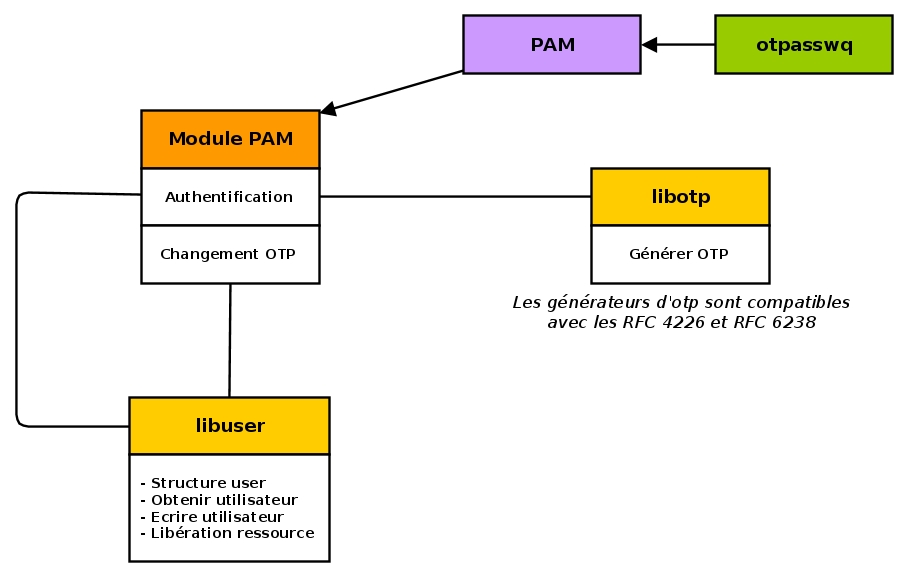
\includegraphics[scale=0.3]{../graphics/architecturepammodule.jpg} 
 
\end{figure}
\end{frame}

\begin{frame}
\frametitle{Android: Interface Utilisateur}
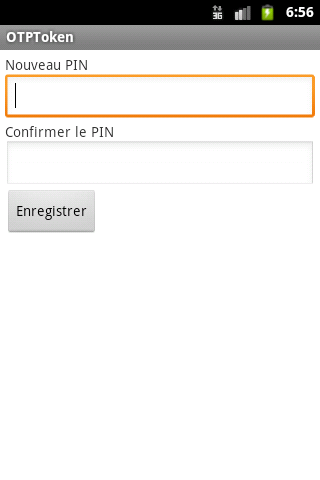
\includegraphics[scale=0.33]{../graphics/enterpin.png}
\hspace{0.8em}
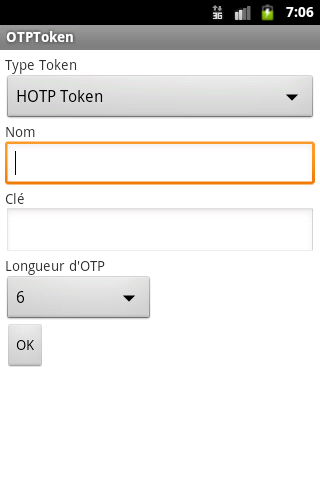
\includegraphics[scale=0.33]{../graphics/firstotp.png}
\hspace{0.8em}
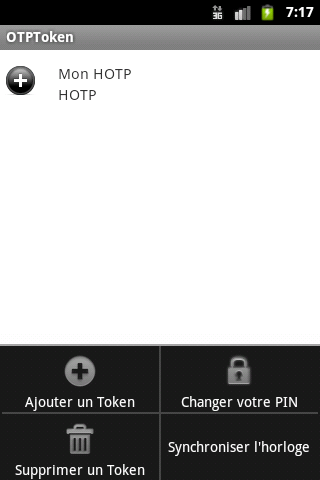
\includegraphics[scale=0.33]{../graphics/menu.png}
\end{frame}

\begin{frame}
\frametitle{Android: Compatibilité}
\begin{block}{API Android}
Level 10: Compatbile avec Android 2.3.X et supérieur.
\end{block}
\begin{block}{Prérequis Matériels}
\begin{itemize}
\item CPU: 700Mhz minimum.
\item Ram: 128Mo minimum.
\end{itemize}
\end{block}
\begin{block}{Google Authenticator}
Notre application est compatible avec les modules Google.
\end{block}
\end{frame}


\begin{frame}
\frametitle{Android: Bibliothèque OTP}
\begin{figure}
 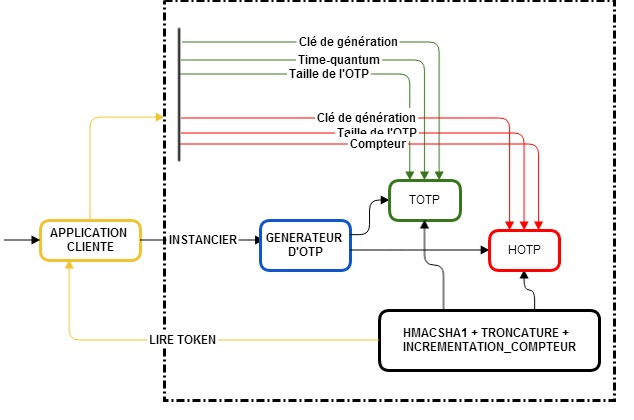
\includegraphics[scale=0.3]{../graphics/libotp-android.jpg} 
\end{figure}
\end{frame}

\begin{frame}
\frametitle{Android: Sécurité des données}
\begin{itemize}
\item Code Pin pour protéger l'accès à l'application.
\item Haché du Pin (avec un sel) dans un fichier.
\item OTP stocké dans un fichier chiffré en AES-256.
\item Nettoyage des fichiers à la désinstallation.
\end{itemize}
\end{frame}





\begin{frame}
\frametitle{Android: Architecture logicielle}
\begin{figure}
 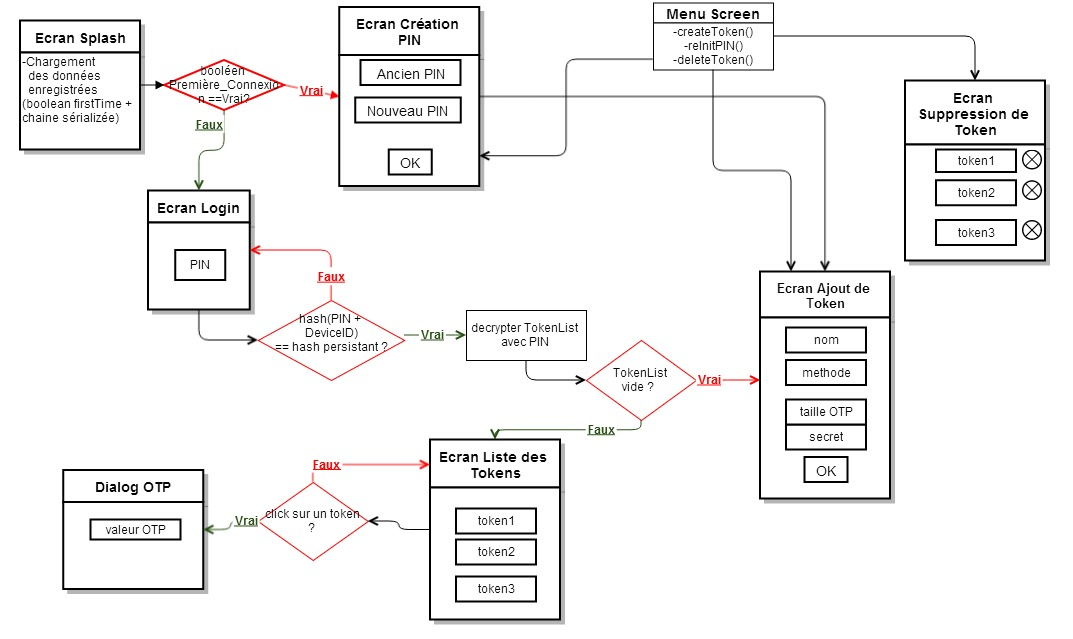
\includegraphics[scale=0.3]{../graphics/archi-android.jpg} 
\end{figure}

\end{frame}


\section{Bilan}

\subsection{Démonstration}
\begin{frame}
\begin{center}
\Huge{Démonstration}
\end{center}
\end{frame}


\subsection{Problèmes rencontrés}
\begin{frame}{Problèmes rencontrés: Gestion}
\begin{block}{Péritonite}
Pas de javacard
\end{block}

\end{frame}


\begin{frame}
\frametitle{Problèmes rencontrés: Android}
\begin{block}{Manifeste}

\end{block}

\begin{block}{Synchronisation}

\end{block}
\end{frame}

\subsection{Tests finaux}
\begin{frame}
\frametitle{Résultat des tests finaux}
\begin{block}{Temps requis pour générer 100 mots de passe}
\begin{itemize}
\item Attendu: \textless  100s
\item Obtenu: 52ms
\end{itemize}
\end{block}
\begin{block}{Temps requis pour vérifier 1 mot de passe}
\begin{itemize}
\item Attendu:\textless  2s
\item Obtenu: 1/100s
\end{itemize}
\end{block}
\begin{block}{Mémoire utilisée pour générer un mot de passe}
\begin{itemize}
\item Attendu: \textless  10ko
\item Obtenu: 7ko
\end{itemize}
\end{block}

\end{frame}

\begin{frame}
\frametitle{Résultat des tests finaux}
\begin{itemize}
\item Résistant au rejeu.
\item Résistant aux attaques exhaustives.
\end{itemize}

\end{frame}

\subsection{Licence}
\begin{frame}
\frametitle{La licence choisie}
\begin{center}
\Huge Creative Commons
\end{center}
%A étoffer + logos

\end{frame}


\section{Conclusion}

\begin{frame}  
\frametitle{Plan} 
\tableofcontents[currentsection,hideothersubsections]
\end{frame}

\begin{frame}
\frametitle{Enseignements tirés du projet}
\begin{itemize}
\item Maitrise de PAM.
\item API Android.
\item Gestion de projet.
\end{itemize}
\end{frame}


\begin{frame}
\frametitle{Améliorations possibles}
\begin{itemize}
\item HOTP en challenge/response.
\item Token sur Java Card.
\end{itemize}
\end{frame}

\begin{frame}
\frametitle{Conclusion}
\begin{itemize}
\item Un projet dans l'ère du temps.
\item Un panel de connaissances variées.
\item Une première expérience de gestion de projet.
\end{itemize}
\end{frame}













\end{document}

